%!TEX root=../paper.tex

\chapter{Timing Margin: A Perpetual Role in \\Modern Microprocessors}
\label{sec:background}

This section explains the basics of microprocessor's timing margin, and motivates why active management of timing margin is necessary to improve power efficiency. This section first goes over the necessity of timing margin in modern microprocessors. Then it enumerates the main components involved in timing margin. We end this section with a brief discussion of the working mechanism of active timing margin.

\section{The Importance of Pipeline Timing Margin}
\label{sec:background:importance}

Timing margin is a necessary component in modern microprocessors, whether it is a general purpose CPU, Graphics Processing Unit (GPU), or specialized accelerators like Tensor Processing Unit (TPU)~\cite{jouppi2017datacenter}.  

Almost all today's processors are pipelined for higher instruction throughput and workload performance. All pipeline stages have the same time duration to complete their computing, or circuit toggling tasks, synchronized by a global clock signal. Each cycle, circuits constructed by CMOS transistors take some time to switch and then produce a stable output electric level to be fed into latches, or registers. Ideally, the circuit's switch time can be calculated, or simulated using CMOS device's charge and discharge time formula given certain supply voltage levels and transistor parameters, and pipeline cycle time should be equal to the simulated switch time, if all pipeline stage have balanced design and have the same switch time. 

However, in practice pipeline circuit's switch time have a lot of uncertainty. The uncertainty of pipeline timing can be caused by, for instance, transistor performance variation due to environment temperature variation, unstable supply voltage levels delivered to the transistors, and imperfect transistor size caused by manufacturing lithography, transistor aging, etc. These sources of timing  uncertainty make circuit switch time deviate from their simulated normal points, which could make circuits complete their jobs faster, or slower than design simulation. To assure all circuits have plenty of time to complete their toggling, pipeline cycle time is always longer than the theoretical circuity switch time, the added time duration in clock cycle is called \textit{timing margin}, as illustrated in~\Fig{fig:timing-margin}. 

\begin{figure}[ht!]
\centering
\subfloat[Timing margin is the time left in clock cycle after circuit completes its work.] {
  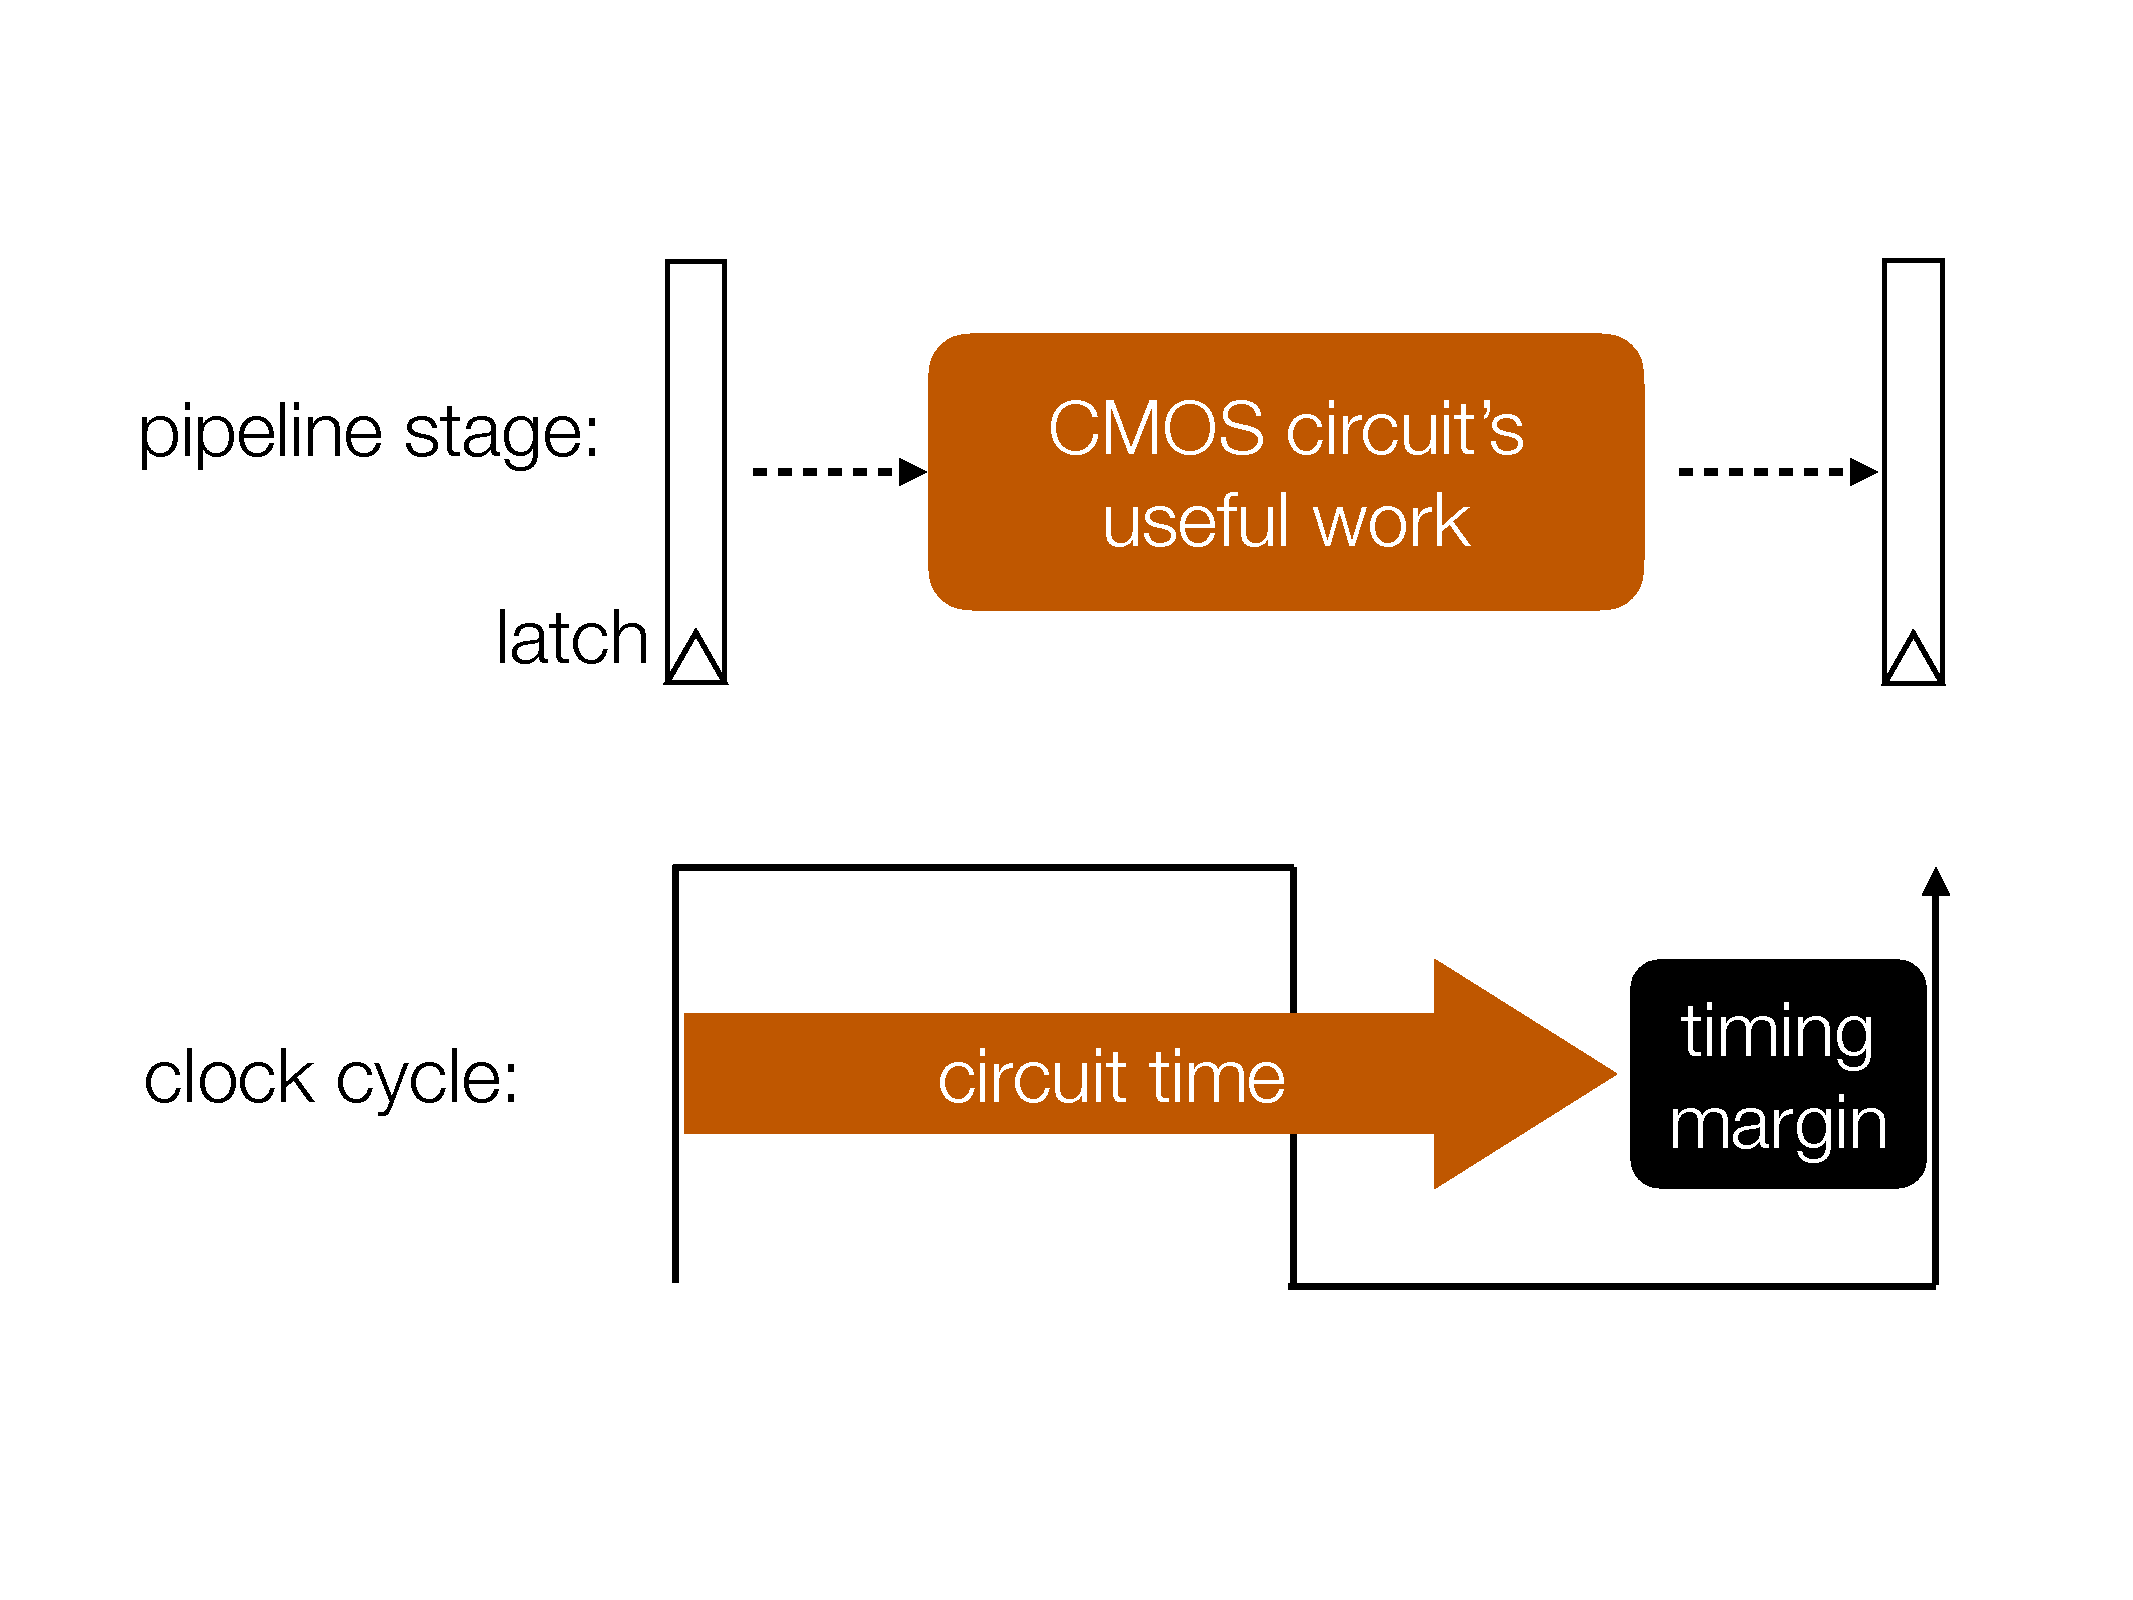
\includegraphics[trim=0 100 0 100,clip,width=0.9\linewidth]{graphs/background/timing_margin.pdf}
  \label{fig:timing-margin} 
}
\\
\subfloat[Voltage guardband] {
  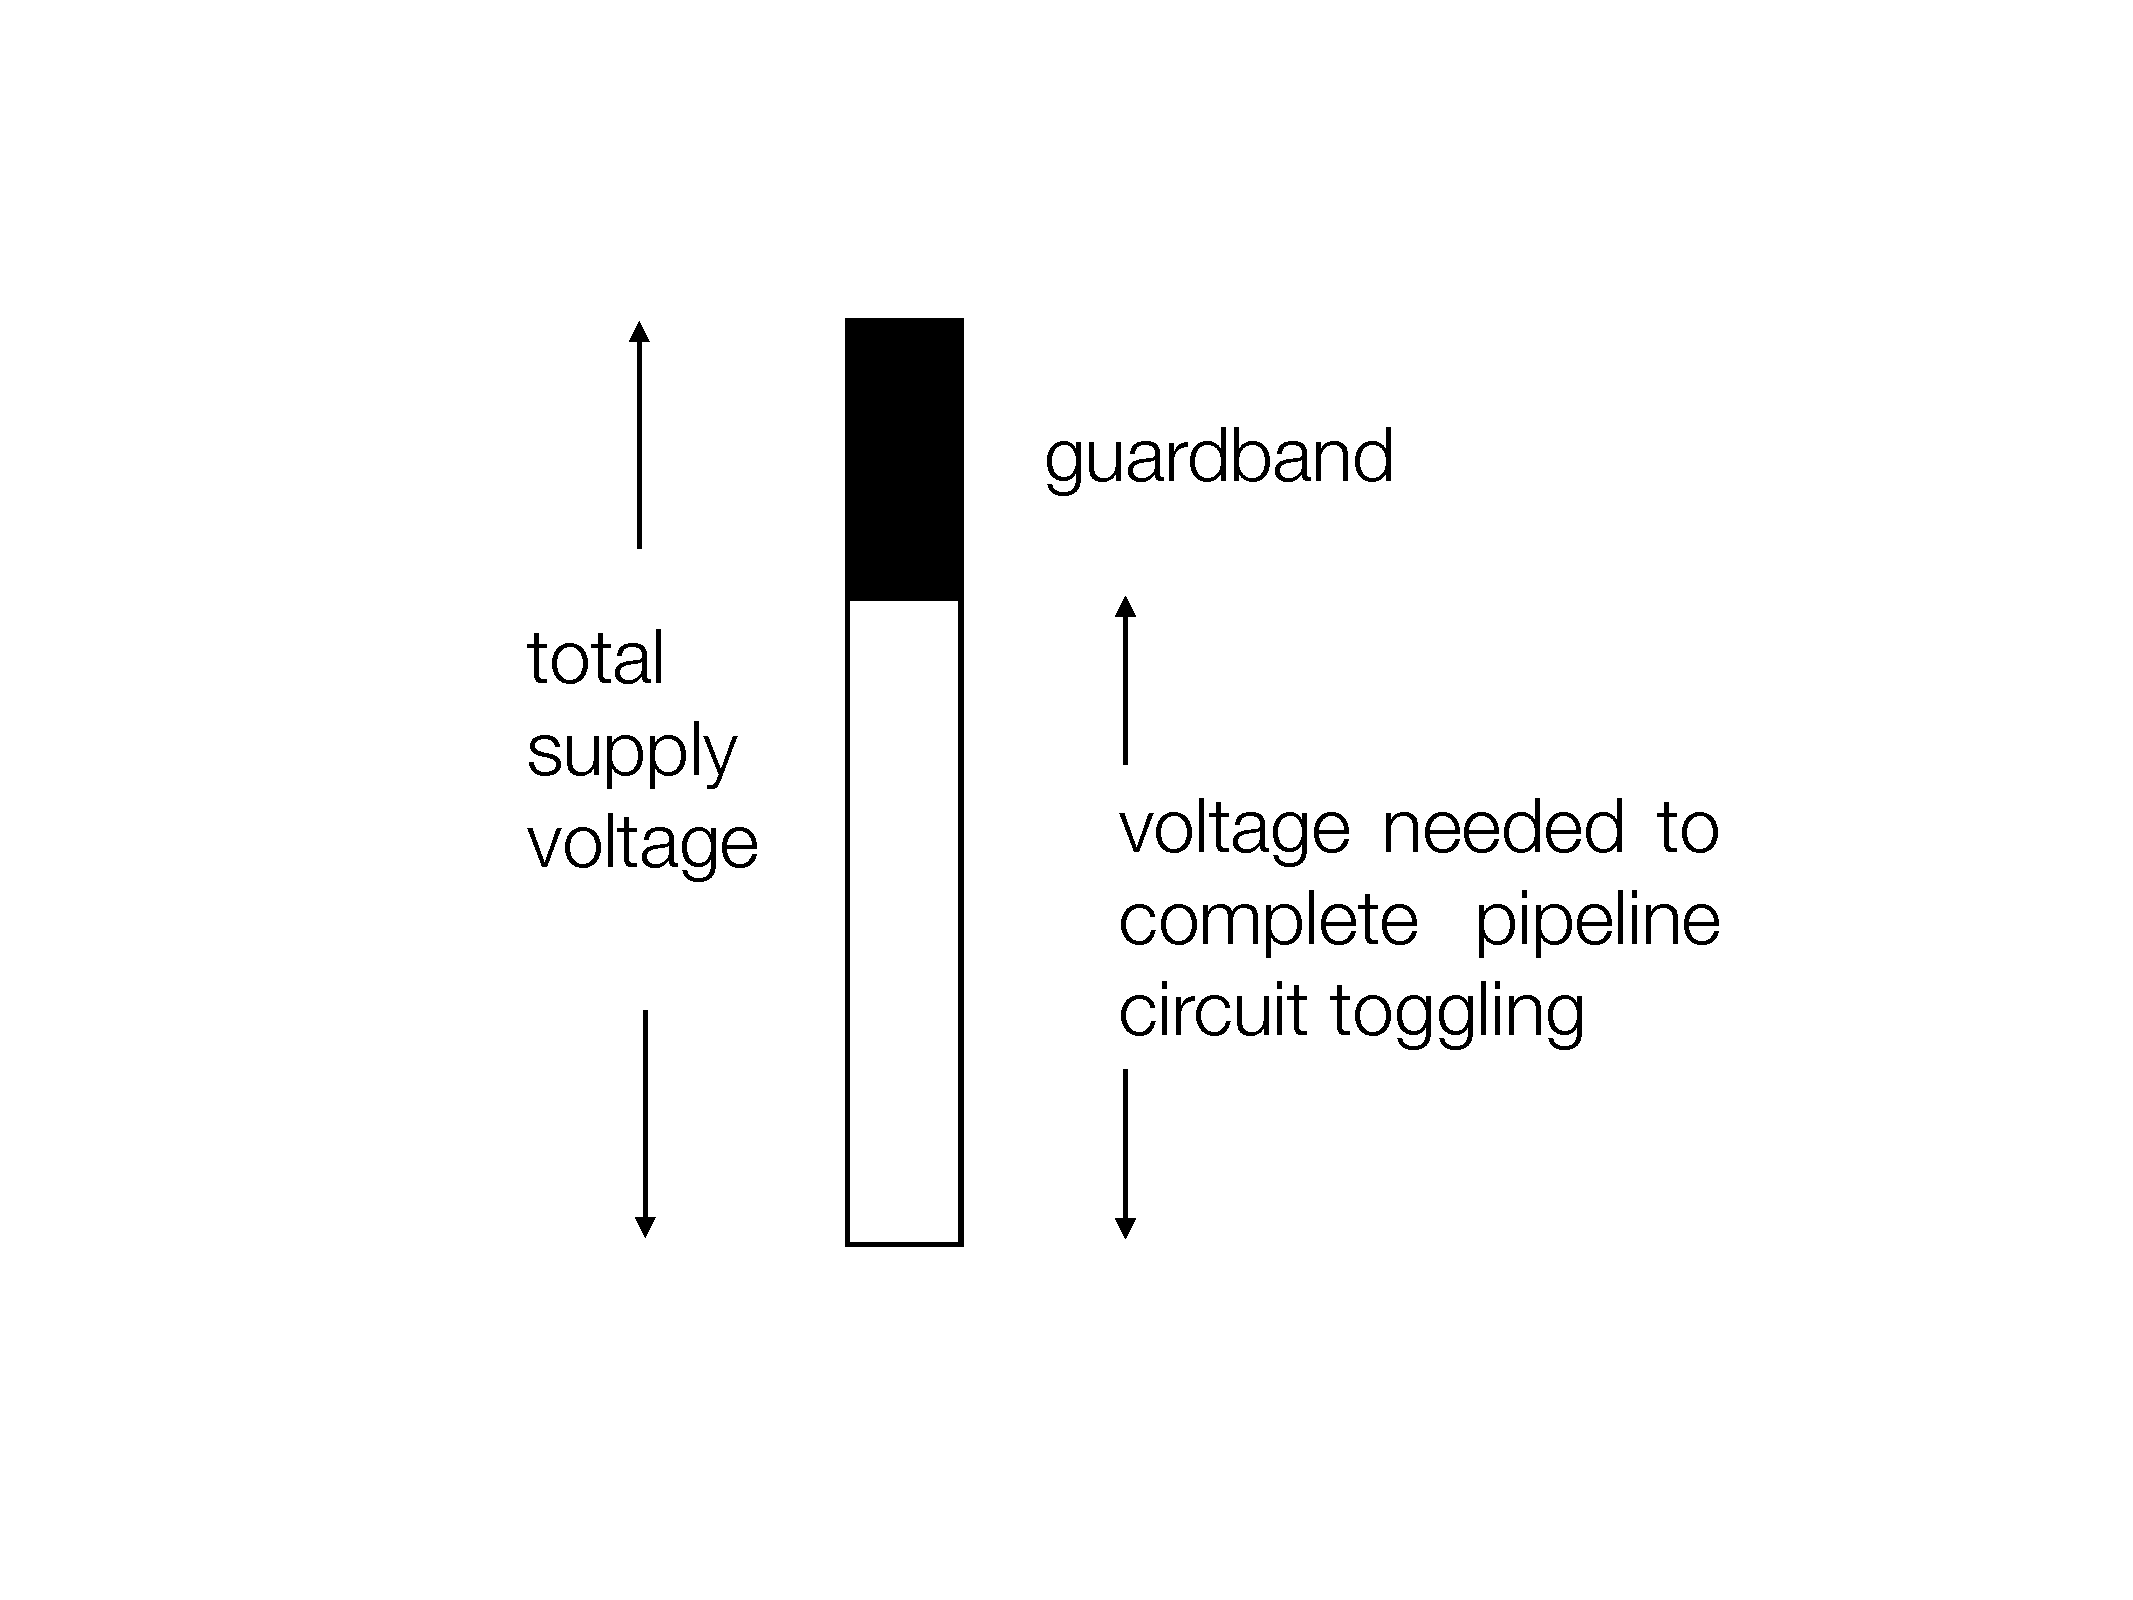
\includegraphics[trim=200 50 200 50,clip,width=.4\linewidth]{graphs/background/voltage_guardband.pdf}
  \label{fig:voltage-guardband} 
}
\subfloat[Power/Performance saving] {
  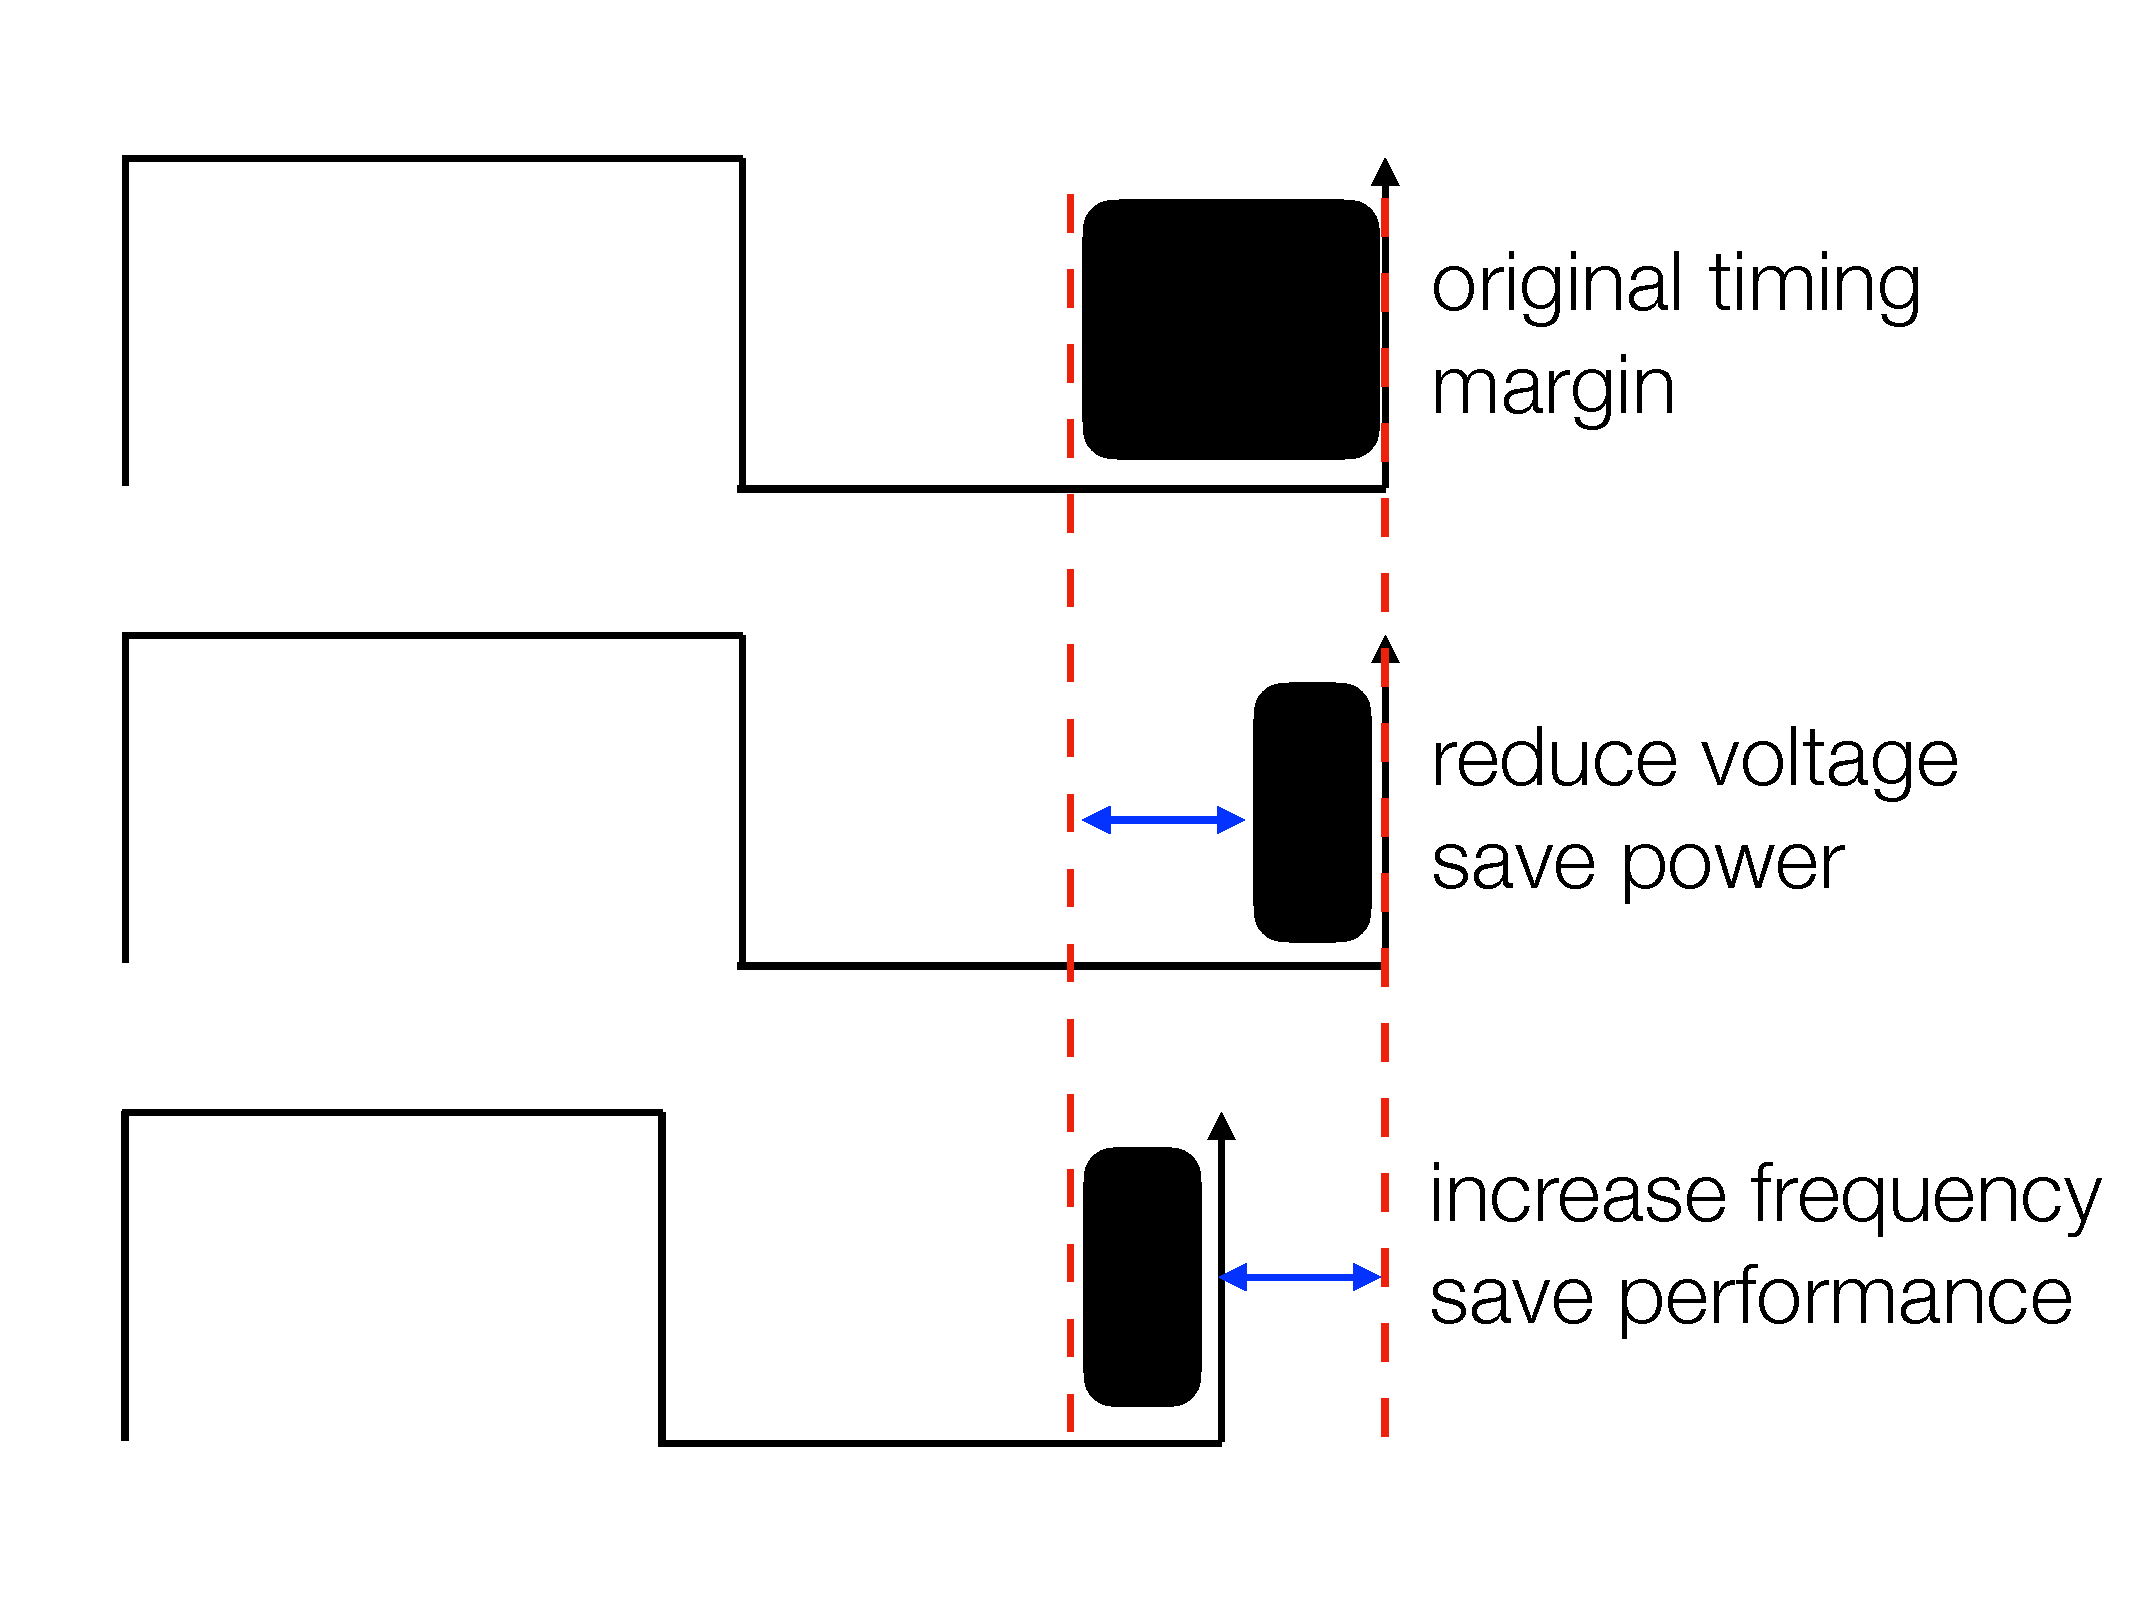
\includegraphics[trim=0 0 0 0,clip,width=.6\linewidth]{graphs/background/saving.pdf}
  \label{fig:adaptive-margin} 
}
\caption{Timing margin ensures processor execution correctness by allocating extra room in pipeline's clock cycle time. Timing margin can be delivered by providing extra voltage, known as the voltage guardband, or alternatively slowing down frequency. Safely reducing the timing margin can improve power via undervolting, or improve performance via overclocking.}
\end{figure}

Timing margin can be implemented as tuning supply voltage higher while leaving frequency target untouched, which makes circuits operator faster and thus leaving margin in the cycle time, or tuning the frequency slower while leaving supply voltage the same, which makes cycle time longer and creating margin. These two methods are equivalent. The former approach is widely known as \textit{voltage guardband} as described in \Fig{fig:voltage-guardband}. In this thesis, we explore opportunities in both designs, i.e., reduce voltage to save power in a voltage guardband approach, and increase frequency to improve performance in a under-clocking approach.

A good analogy of microprocessor pipeline's timing margin in everyday life is the relationship between cars and lanes. Ideally, a lane would have the same width as a car if cars can strictly run according to the orbits of the lane. Yet, in reality, lanes are always much wider than cars because cars often deviate from lane orbits. The deviation uncertainty may be caused by human driver's improvisation, or the inherent control error of the vehicle (e.g., a mismatch between the left and right tires). The extra space between a lane and a car allows tolerates these errors and make sure no accidents occur. The extra room between lane width and car width works just like how pipeline timing margin protects against circuit's timing uncertainty.

Failing to provide enough timing margin is catastrophic for modern processors as it can lead to pipeline timing errors, causing incorrect application execution results, or even system crash. Circuits need enough time to deliver the correct signal for the next pipeline stage to compute on. With not enough margin, the circuit may not have enough time to produce the correct bit, due to unusual load environment like extreme temperature environments. The erroneous bits can be meaningless, pointing to a wrong data address, or representing an invalid instruction that cannot be decoded, breaking microprocessor's correct execution stage.

This dissertation addresses the timing margin issue on processor, primarily CPUs and GPUs. However, timing margin widely exists on other kinds of chips that use pipeline microarchitecture, and are equaly important to guarantee correct chip functioning. One intuitive example is the rowhammer in DRAM chips~\cite{kim2014flipping}. The authors in~\cite{kim2014flipping} found that stressing one row in DRAM chips can cause adjacent row's cells to have erroneous bit storage. The underlying mechanism is because frequency access to a row creates local temperature hotspot, which makes DRAM cell capacitor to leak charge quicker than designed bit retention period. To protect against this situation, DRAMs need to allocate more margin to bit refresh frequency, making sure the cell's charge leakage time do not exceed the threshold for retaining the correct bit in the worst runtime environment. Though DRAM is not exactly the same as a microprocessor's logic circuit structure, this case illustrates the importance of timing margin in pipelined chips.

\section{What Consumes the Timing Margin?}
\label{sec:background:components}

Timing margin is excessively high in today's processors, costing over 20\% extra supply voltage in shipped chips~\cite{reddi2010voltage, leng2015gpu}. Our work, along with many prior art tries to reduce timing margin magnitude and saves power or performance. The first step to achieve this goal is to understand what timing margin is allocated for, or at runtime what phenomenon makes pipeline circuit time deviates from normal and erodes, or consumes the margin. Although the uncertainty in pipeline circuit timing are caused by parasitic effects in the computer system, they are not completely random. In this dissertation, we dissect modern processor's timing margin into three main components, allocated for different consuming effects, namely temperature, voltage, and process variation (TVP variation~\cite{reddi2013resilient}). We believe these three effects are the biggest consumers that contribute to timing margin's high amount, and they happen mostly in independent manners which facilitate us to optimize them one by one.

\paragraph{Temperature variation} is one important source of timing uncertainty. When temperature changes, transistor performance varies because temperature variation alters the activity level of the particles flowing in CMOS transistor's channel, which changes transistor switch speed and circuit completion time. In practice, processor temperature variation is unavoidable because during workload run the charge and discharge of semiconductor transistors inevitably raises temperature. Depending on workload intensity, the temperature profile of the chip varies temporarily and spatially, affecting circuit timing. To tolerate timing uncertainty caused by temperature variation, margin must be added in the cycle time. In \Sec{sec:temperature} we perform an in-depth study on how temperature affects timing margin, and propose a feedback loop with corresponding management to combat against it.

\paragraph{Voltage variation} is a very dangerous source of timing uncertainty. It is caused by the interaction between the parasitics of the power delivery subsystem of a microprocessor and the processor's varying power draw under workload execution. \Fig{fig:pdn-model} from~\cite{leng2014gpuvolt} gives an intuitive overview of the electrical mechanism of voltage variation.

\begin{figure*}[t!]
  \centering
  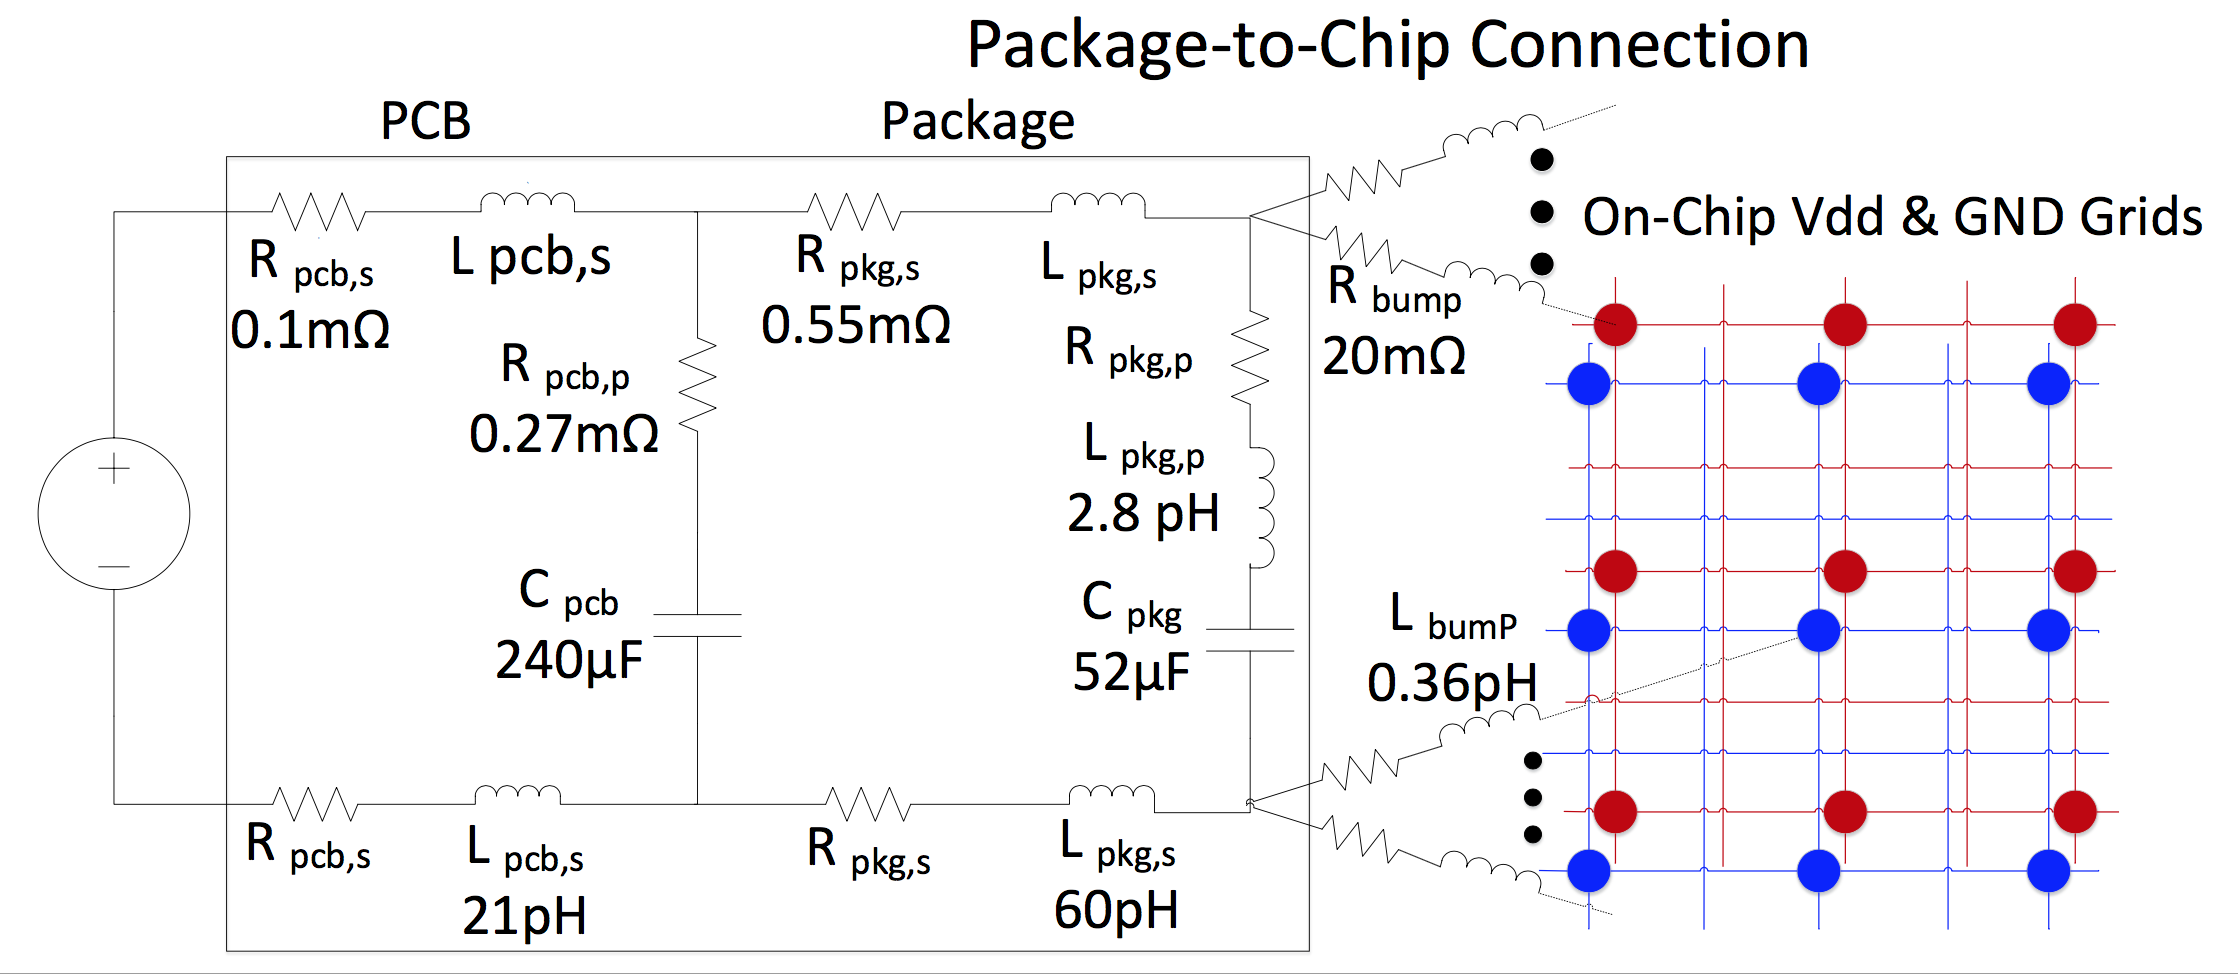
\includegraphics[trim=0 0 0 0,clip,width=0.8\linewidth]{graphs/background/pdn-model.png}
  \caption{An electrical model of a computer's power delivery subsystem, from the voltage regulator module (VRM) to on-chip transistors. Resistive, capacitive, and inductive impedance exist on this path, adding noise to the voltage delivered to transistors which causes timing uncertainty.}
  \label{fig:pdn-model}
\end{figure*}

The supply voltage delivered to the CMOS transistors contains lots of noise because the path from the source of voltage supply to the end transistors has electrical parasitics, including resistive, capacitive, and inductive components. Typically, the power supply subsystem can be modeled as four parts: the voltage regulator module (VRM), the printed circuit board (PCB), the package, and on-die power delivery network (PDN). Each part contributes to the total impedance. These impedance exist because the power delivery subsystem is made of real, physical materials - on-chip and off-chip wires have resistance even the magnitude can be small, wires can form loops by chance and create inductive impedance, the alignment between wires and the added decoupling capacitors create capacitance, etc.

Resistive parasitics cause supply voltage's IR drop following Ohm's law. Higher power causes higher IR drop. Inductive and capacitive parasitics further worsen supply voltage with the $di/dt$ effects. $di/dt$ effect happens when there is rapid change in the current draw, or power consumption of the transistors. $di/dt$ effect is happens rapidly, typically over tens of cycles, yet very rarely, making it hard to tract. The combined IR drop and $di/dt$ effects make the supply voltage experienced by transistors very noisy, adding uncertainty to circuit timing. In \Sec{sec:voltage}, we perform in-depth analysis on how state-of-the art hardware tries to reduce voltage noise and propose management techniques to squeeze out power efficiency from voltage noise.

\paragraph{Process variation} is another source of uncertainty if pipeline circuit timing. Unlike temperature and voltage variation which change dynamically during runtime, process variation is a static effect that is formed during chip's manufacturing lithography process. During lithography, transistor performance variation occurs because the lithography instruments cannot perfectly control the various lithography steps, such as etching and doping. Wire width, transistor gate width and length can be etched with noise. Dopant density can deviate from the ideal density level. All these effects make transistor and wire's performance deviate from the ideal case, and make the speed of different transistors and wires differ. A microprocessor's performance is determined by the slowest part of the chip. The result is that faster circuits are forced to have some amount of timing margin because it is synchronized using the same clock as the slow circuits. In \Sec{sec:process} we devise automatic methods to expose a multicore's performance variation caused by process variation, and propose management schemes to manage the resulting non-deterministic application performance.

We acknowledge there are other effects that also contribute to the timing margin, such as transistor aging and processor testing inaccuracy. However, these effects are not as strong as the temperature, voltage, and process variation aforementioned in a processor's typical lifetime, and the condition for it to occur is too extreme. For this reason, we leave out these effects in this dissertation.

\section{The Need for Active Timing Margin}
\label{sec:background:motivation}

While it is intuitive to allocate timing margin in pipeline cycles to combat various effects that cause circuit timing uncertainty, the specifics of how the amount of margin is calibrated is intricate. 

In traditional designs, the margin is estimated during chip design and testing stage, following a \textit{worst-case} design approach. Under this approach, the amount of timing margin is a static value that is able to tolerate the most extreme conditions that slow down microprocessor circuits, such as very heavy $di/dt$ voltage droops, very large IR drop caused by high power workloads, and unusual operating temperature that degrade transistor performance significantly. Because timing margin is a fixed value in this design, failing to consider all corner cases or allocating margin not conservatively enough may neglect an extreme corner case the user might create to hamper pipeline timing. Thus, the static worst-case timing margin must aggregate corner case of all effects to determine the total amount of margin is added to the chip.

The cost of the worst-case margining approach, however, is prohibitively high despite its straightforward and low-overhead implementation. Prior art has shown that the extreme conditions that will utilize all the margin happens extremely rarely, for voltage noise the heavy $di/dt$ droops over 10\% of the supply $V_{dd}$ happens less than 1\% of the time~\cite{reddi2010voltage, leng2014gpuvolt}, while timing margin must protect against these rare worst cases, leaving the margin unused most of the time. In~\cite{leng2015safe}, researchers reported that 20\% of the supply voltage of a commercial GPU can be safely reduced without causing program execution errors, which reflects the huge amount of voltage guardband and timing margin in today's chips. These wastage is significant not only because of the power and energy wasted, but also because today's microprocessors are inherently power limited, and wasting power means limiting processor performance. Therefore it is imperative that we investigate what leads to timing uncertainty and consumes timing margin.

Many research efforts have been made to reduce the magnitude of the conventional static worst-case margin, ranging from benchmarking and simulation efforts to understand the worst-case limit~\cite{kim2012audit,bertran2014voltage, sarangi2008varius}, microarchitecture analysis to characterize the events that lead to rare extreme noise conditions~\cite{powell2003pipeline, gupta2007understanding, gupta2009event, reddi2009voltage}, low-overhead architecture design for error toleration and noise smoothing~\cite{gupta2008decor,reddi2009voltage,leng2015gpu, ernst2003razor}, to software techniques including compilation, scheduling, and runtime management to avoid high timing margin consumption~\cite{reddi2010eliminating,miller2012vrsync,papadimitriou2017harnessing,leng2015safe}. Many of these works have shed useful insights and are partly incorporated into latest designs. However, most of these proposals are not adopted as a whole by industry, either because of their high design overhead, lack of reliability guarantee, or unacceptable performance overhead.

This dissertation concentrates on one particular design flavor widely adopted for reducing timing margin, \textit{Active Timing Margin}. The idea of active timing margin is very intuitive - instead of providing margin for the worst case, active timing margin provides just enough margin under the present condition, and dynamically stretches the margin when emergent event occurs, whether temperature goes to extreme, voltage falls very low, or threads are running on a flow core. Active timing margin relies on environment sensors to check runtime load conditions, including timing margin sensors, temperature sensors, power sensors, etc, rather than performance event counters to predict when a high-stake event may occur as the cost of misprediction can be high. 

\begin{figure}[t!]
\centering 
  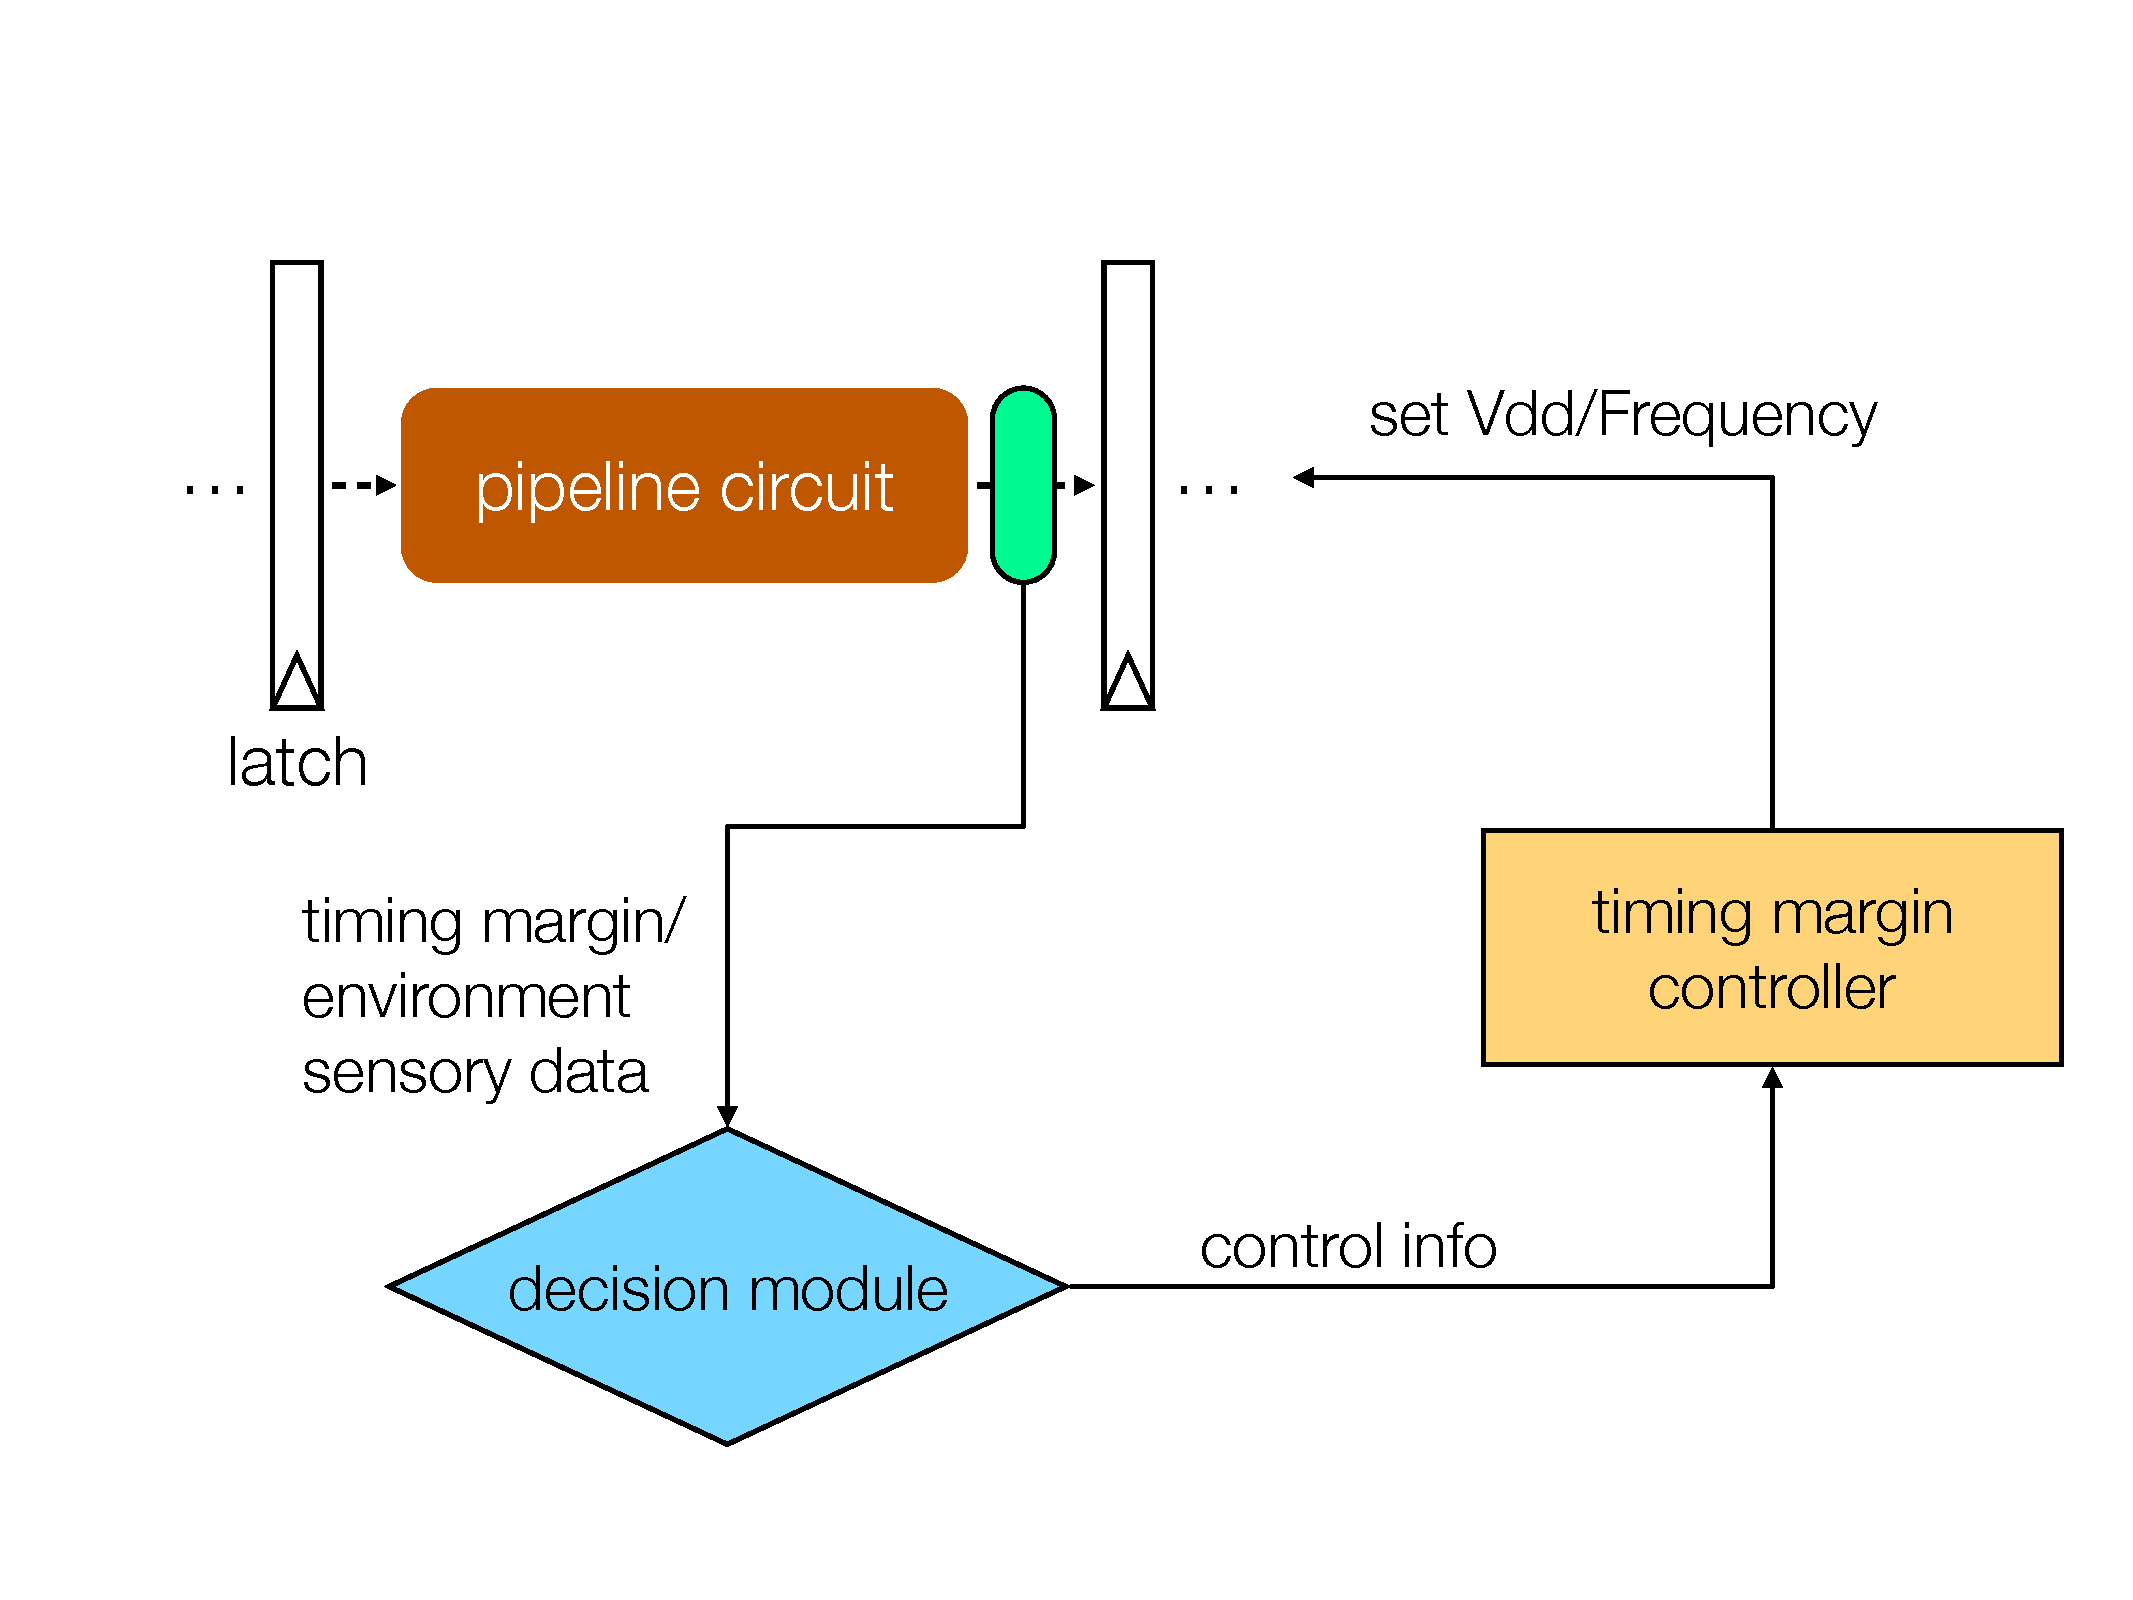
\includegraphics[trim=0 0 0 0,clip,width=0.9\linewidth]{graphs/background/atm.pdf}
  \caption{Active timing margin is a control loop that detects timing margin and related chip load environment, and accordingly adjust supply voltage or operating frequency in real-time to supply just enough margin.}
  \label{fig:atm-example}
\vspace{-0.2in}
\end{figure}

\Fig{fig:atm-example} illustrates a high-level design of active timing margin. It uses a control loop between the sensor and the voltage/frequency controller to adjust chip timing margin based on real-time monitored load environment. Because active timing margin has very low design and verification overhead, and it has been proven to be effective in mitigating process, voltage, and temperature variation, active timing margin has been become the de facto approach for modern chips to reduce margin~\cite{efurgy2011active, bowman201222nm, tokunaga20145,grenat20145,bowman20158,webel2015robust,vezyrtzis2018droop,zu2016tistate}.

\begin{figure}[t!]
\centering 
  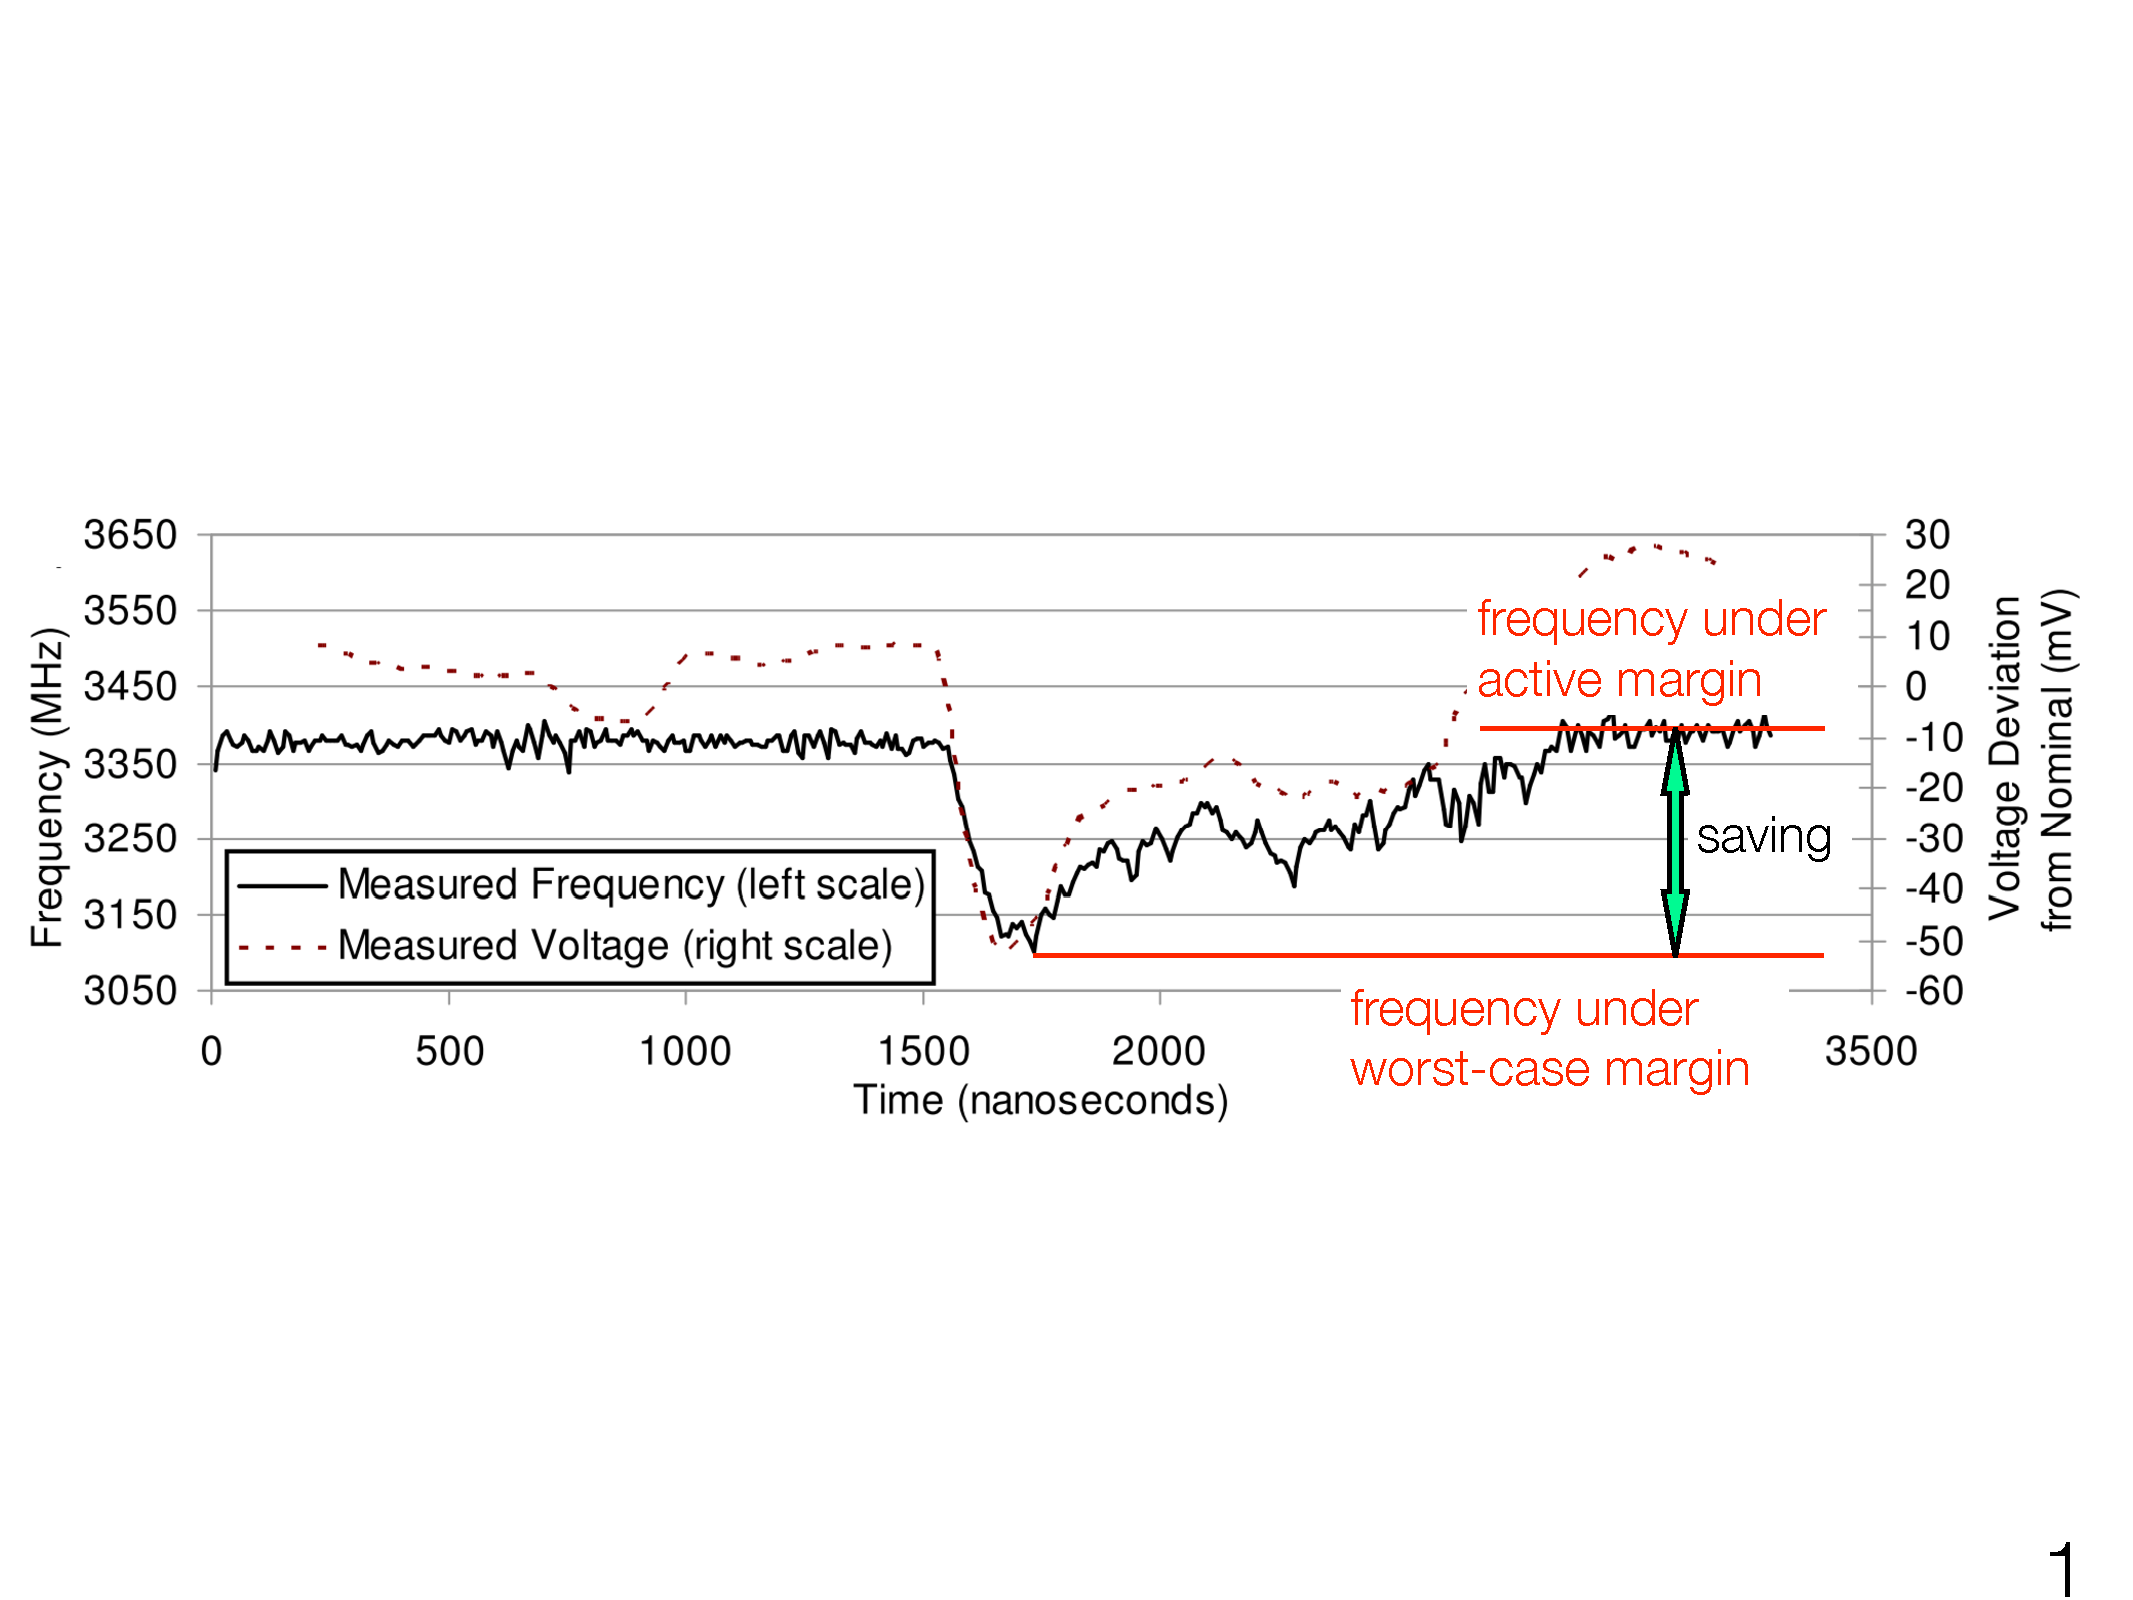
\includegraphics[trim=0 200 0 200,clip,width=0.95\linewidth]{graphs/background/example.pdf}
  \caption{Active timing margin protects $di/dt$ effect by making frequency/clock cycle track supply voltage, which improves performance and reduces timing margin wastage.}
  \label{fig:didt-example}
\vspace{-0.2in}
\end{figure}

\Fig{fig:didt-example} from~\cite{lefurgy2011active} illustrates how active timing margin deals with the dangerous $di/dt$ effect. Starting at 1500~ns, a heavy voltage droop caused by strong $di/dt$ effect slows down circuits, and necessitates some amount of timing margin to protect against it, losing performance under the same supply voltage. The static margin needs to set at the lowest frequency at 3050~MHz to tolerate the $di/dt$ effect. However, only small voltage ripple occurs on the power delivery network when heavy $di/dt$ effect is over. During these periods, large timing margin is not needed, yet the static approach still provisions the timing margin set by the worst case, wasting a lot of performance under the same voltage. 

To reclaim the wasted frequency, active timing margin dynamically adjust clock frequency to match the magnitude of voltage variation. When the $di/dt$ effect occurs, clock frequency ramps down quickly to provide the need timing margin. When there's no $di/dt$ effect, clock frequency stays at a higher level to reclaims the unused timing margin. Overall, the system enjoys higher performance.